\section{Evaluation}
\label{sec:experiments}

This section evaluates the effectiveness of \tool through standalone experiments and end-to-end distributed machine learning scenarios of data, model, and pipeline parallelism.

%\subsection{Experimental Setup}
Our experiments are performed on a cluster of 16 NVIDIA DGX-2 nodes where each node contains dual 24-core Intel Xeon CPUs and 16 NVIDIA Tesla V100 (32GB) GPUs.
%with 32 GB of memory for each. 
Each GPU within a node is connected to six NVSwitches with six NVLinks (25~GBps per NVLink).
Nodes are connected with 8 non-blocking EDR InfiniBand (100~Gbps) network.
All nodes run Ubuntu 20.04, CUDA~11.3, cuDNN 8.2 and PyTorch 1.10.

\subsection{Data Parallel Training}
In data parallelism, communication involves an \allreduce of gradients among all ranks. The output is used by the optimizer to update the model parameters.  We evaluate \tool generated code for two widely-used optimizers, Adam and LAMB.
All our experiments in this section were performed on all 16 DGX-2 nodes in our cluster.

\subsubsection{Standalone Experiments}
We first perform standalone experiments to explore different \tool schedules over a range of input tensors from $2^{10}$ to $2^{30}$ elements.
The autotuner generates and executes implementations with different configurations, including all NCCL protocols and all channels from 2 to 64.
For each tensor, the autotuner reports the best average result of 1000 iterations.

\spara{Baselines} The baselines perform parameter update by first doing \allreduce over gradients and then call FusedAdam or FusedLAMB from NVIDIA Apex~\cite{apex}. 
Both FusedAdam and FusedLAMB fuses all the parameter update computations.
% \tool additionally provides the ability to fuse such computation with the \allreduce kernel.
% FusedAdam and FusedAdam are written in 6.2K lines of code, while \tool schedules are roughly $10$ lines of code. 

\spara{\tool Schedules}
The autotuner generates following three schedules of Adam and LAMB by applying different \tool transformations for each input size and reports the best schedule to the user for each input size:
\begin{enumerate}[leftmargin=*,topsep=2pt]
  \item \textbf{AR-Opt} (Opt = Adam/LAMB) refer to the traditional parameter update technique, i.e., an \allreduce over gradients  and then each GPU individually performs the optimizer computation. These schedules fuse all computations into a single kernel, thereby simulating the baseline implementations of FusedAdam and FusedLAMB.
  \item \textbf{GShard-Eq} or \textbf{RS-Opt-AG} (Opt = Adam/LAMB) are generated from \textit{AR-Opt} by first splitting the \allreduce into \reducescatter and \allgather, and then reordering \allgather with the fused optimizer computations.
  Hence, these schedules distribute parameter update across all ranks, similar to GShard~\cite{gshard} and ZeRO~\cite{zero}. Since GShard does not support execution on GPUs, we refer to this schedule as GShard-Eq in our results. 
  %  we evaluate \tool schedules that uses same technique as GShard.
  \item \textbf{fuse(RS-Opt-AG)} (Opt = Adam/LAMB) are generated by fusing all operations of \textit{RS-Opt-AG} into FusedAllReduce.
\end{enumerate}

\paragraph{Results}
%We first presents results for a single contiguous tensor and then for several non-contiguous tensors.
\begin{figure}[t]
	\centering
    \begin{subfigure}{0.93\linewidth}
    \centering
    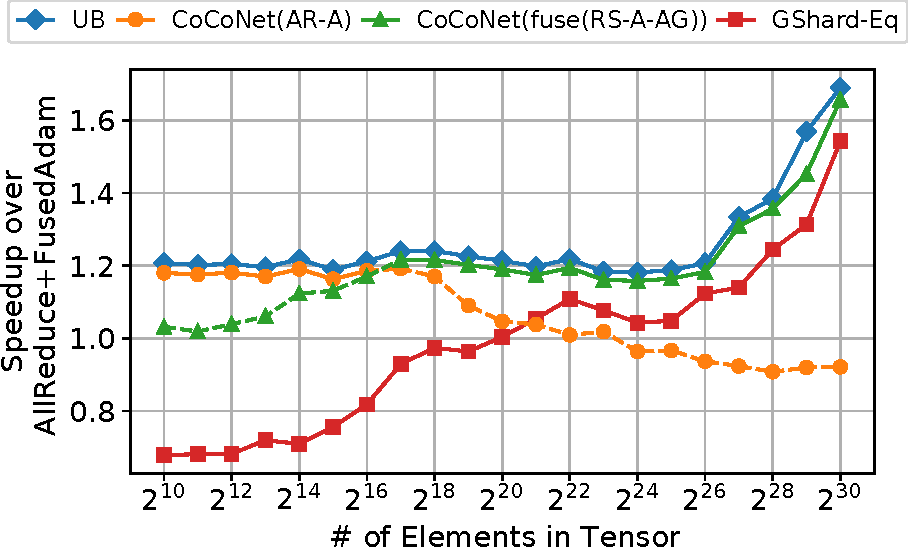
\includegraphics[width=\linewidth]{figures/results-adamfp16-256-gpus.pdf}  
%    \caption{Mixed-precision Adam. AR-A represents AR-Adam and runs best till 2$^{16}$. fuse(RS-A-AG) represents fuse(RS-Adam-AG) and runs best after 2$^{17}$.}
    \caption{Mixed-precision Adam. AR-Adam(AR-A) runs best till 2$^{16}$. fuse(RS-A-AG) represents fuse(RS-Adam-AG) and runs best after 2$^{17}$.}
    \label{fig:bandwidth64GPUs:adam}
  \end{subfigure}
  \par \bigskip% Do not remove this. Without this there is no space between caption of above figure and the next figure. WEIRD bug. Never saw this in subfigure.
  \begin{subfigure}{0.93\linewidth}
    \centering
    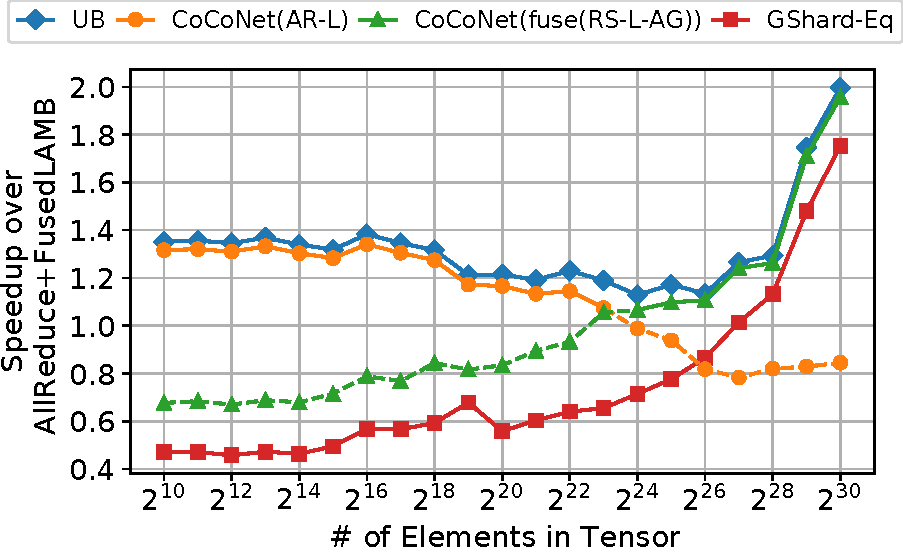
\includegraphics[width=\linewidth]{figures/results-lambfp16-256-gpus.pdf}  
%    \caption{Mixed-precision LAMB. AR-L represents AR-LAMB and runs best till 2$^{16}$. fuse(RS-L-AG) represents fuse(RS-LAMB-AG) and runs best after 2$^{17}$.} 
    \caption{Mixed-precision LAMB. AR-LAMB(AR-L) runs best till 2$^{16}$. fuse(RS-L-AG) represents fuse(RS-LAMB-AG) and runs best after 2$^{17}$.} 
    \label{fig:bandwidth64GPUs:lamb}
  \end{subfigure}
  % \begin{subfigure}{\columnwidth}
  %   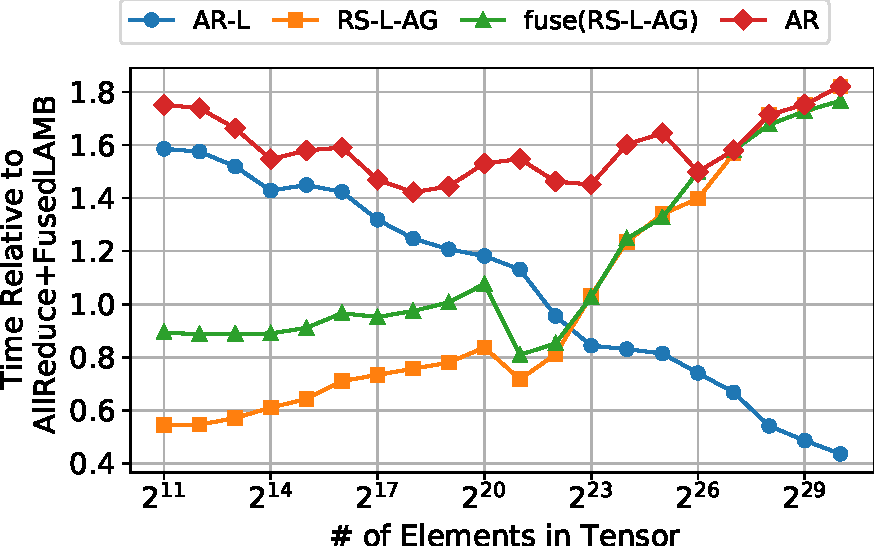
\includegraphics[width=\columnwidth]{figures/results-lambfp16-64-gpus.pdf}  
  %   \caption{Mixed Precision LAMB\label{fig:bandwidth64GPUs:lambmp}} 
  % \end{subfigure}
  \caption{\tool speedup on 256 GPUs. For each size, \tool chooses the best schedules.
   UB (upper bound) takes AllReduce-only as max achievable speedup.
  %  GShard/ZeRO represnts the RS-Adam-AG and RS-LAMB-AG schedules.
   }
  \label{fig:bandwidth64GPUs}
\end{figure}

Figure~\ref{fig:bandwidth64GPUs} shows the speedup of \tool schedules over the baseline
for several tensor sizes. 
The results are shown for mixed-precision~\cite{mixed-precision-training} using Float 16, and the results for Float 32 are qualitatively similar. 
In these figures, UB represents the cost of \allreduce alone without doing any computation, and thus is the upper bound of possible speedups. 

Even though the \textit{AR-Opt} schedules emulate the baseline implementations, they are faster on smaller tensors.
This is because the baseline implementations perform additional preprocessing to optimize the amount of thread-parallelism and instruction-level parallelism per invocation. While this preprocessing cost hurts smaller tensors, its benefit shows up for larger tensors where \textit{AR-Opt} performs worse. 

Since \textit{GShard-Eq} and \textit{fuse(RS-Opt-AG)} schedules distribute the optimizer computation,  they perform better than the baseline for large tensors.
The performance of \textit{fuse(RS-Opt-AG)} shows the advantage of fusing computation and communication kernels as these schedules achieve near optimal speedups for large tensors. 
These schedules are respectively 13\% and 14\% faster than GShard-Eq for Adam and LAMB.

For smaller tensor sizes, multiple kernel calls are required for GShard-Eq schedules significantly hurt performance. Interestingly, \textit{fuse(RS-Opt-AG)} schedules are slower than \textit{AR-Opt} schedules for smaller tensor sizes though they require one less kernel call because the fused kernels have a higher register usage, thereby restricting the thread-level parallelism. This demonstrates that the fusion of communication and computation is not always a good idea.

Table~\ref{tab:loc:data-parallel} shows that the lines of generated code for each schedule are significantly more than the implementation in \tool and the autotuner explored all schedules in 10 seconds.
In summary, \tool provides performance improvements over baselines with fewer lines of code.
The \textit{AR-Opt} and the \textit{fuse(RS-Opt-AG)} reach close to optimal performance for smaller and larger tensors respectively. This amounts to a speedup of 1.2$\times$ to 1.7$\times$ for Adam and 1.35$\times$ to 2.0$\times$ for LAMB.  
There is no schedule that performs best for all sizes, which demonstrates the need for the autotuner. 

\iffalse
\begin{figure*}
  \small
  \begin{subfigure}{0.66\columnwidth}
    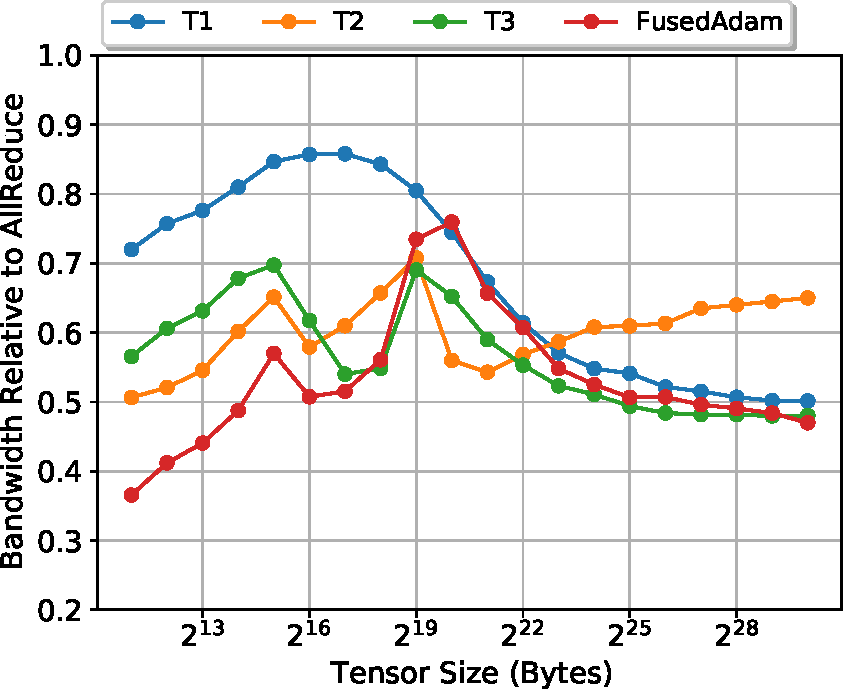
\includegraphics[width=\columnwidth]{figures/results-adam-2-gpus.pdf}  
    \caption{FP32 Adam on 2 GPUs}
  \end{subfigure}
  \begin{subfigure}{0.66\columnwidth}
    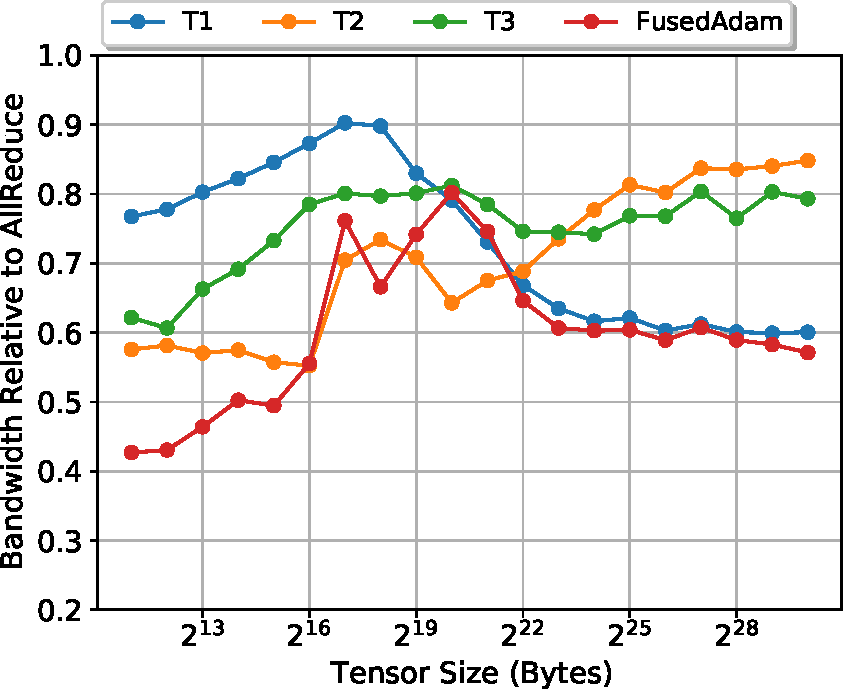
\includegraphics[width=\columnwidth]{figures/results-adam-4-gpus.pdf}  
    \caption{FP32 Adam on 4 GPUs}
  \end{subfigure}
   \begin{subfigure}{0.66\columnwidth}
    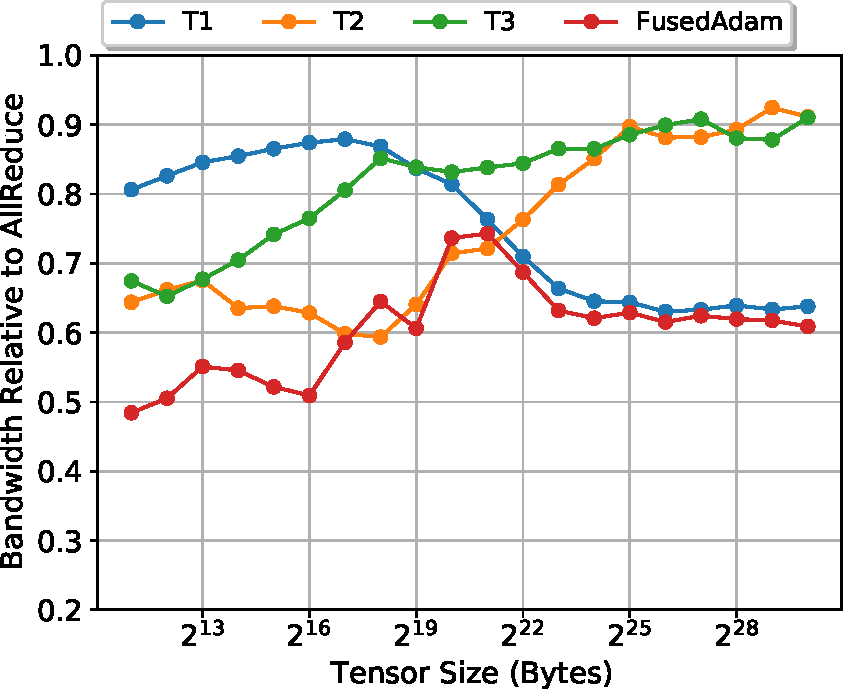
\includegraphics[width=\columnwidth]{figures/results-adam-8-gpus.pdf}  
    \caption{FP32 Adam on 8 GPUs}
  \end{subfigure}

  \begin{subfigure}{0.66\columnwidth}
    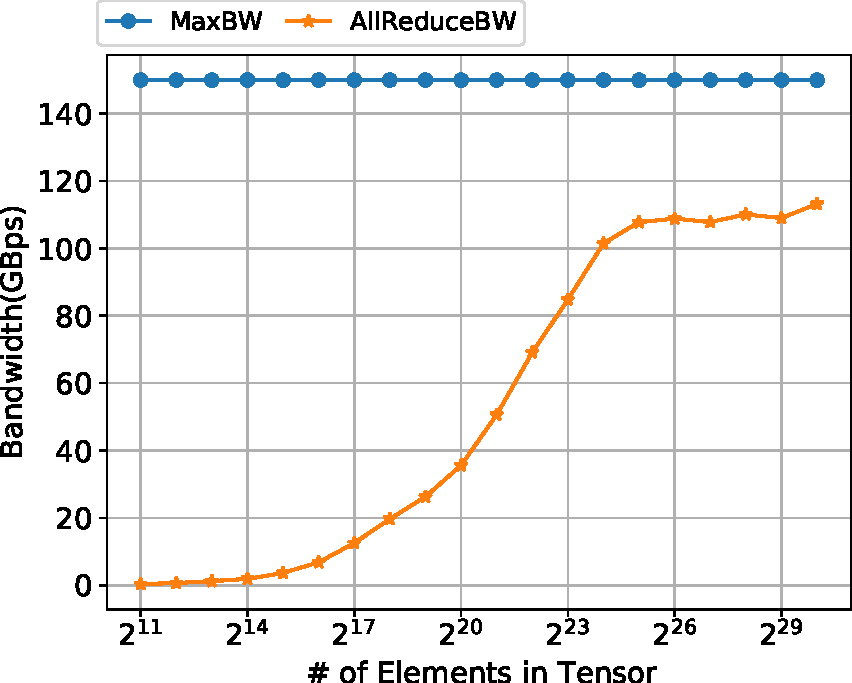
\includegraphics[width=\columnwidth]{figures/results-adam-16-gpus.pdf}  
    \caption{FP32 Adam on 16 GPUs}
  \end{subfigure}
  \begin{subfigure}{0.66\columnwidth}
    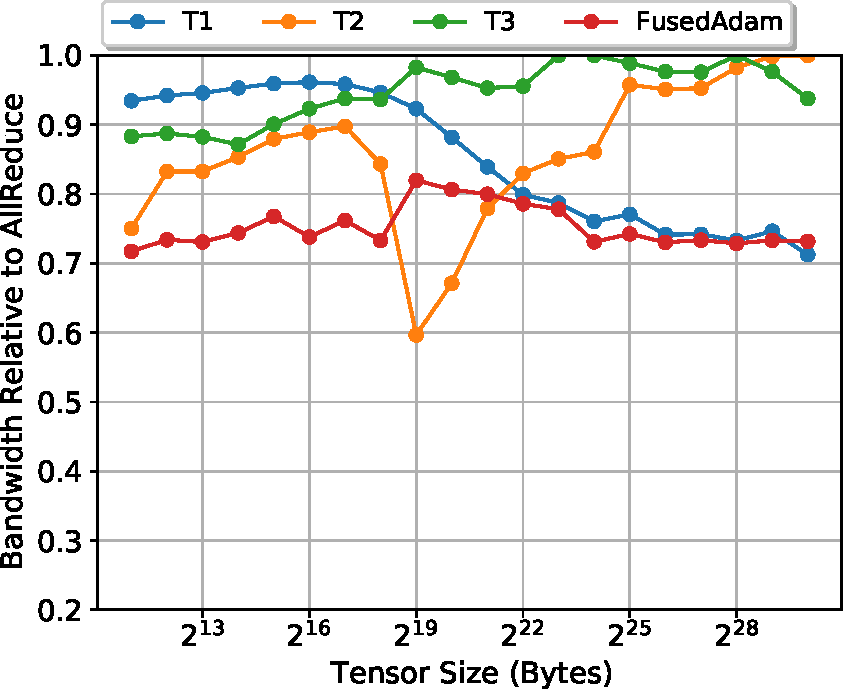
\includegraphics[width=\columnwidth]{figures/results-adam-32-gpus.pdf}  
    \caption{FP32 Adam on 32 GPUs}
  \end{subfigure}
  \begin{subfigure}{0.66\columnwidth}
    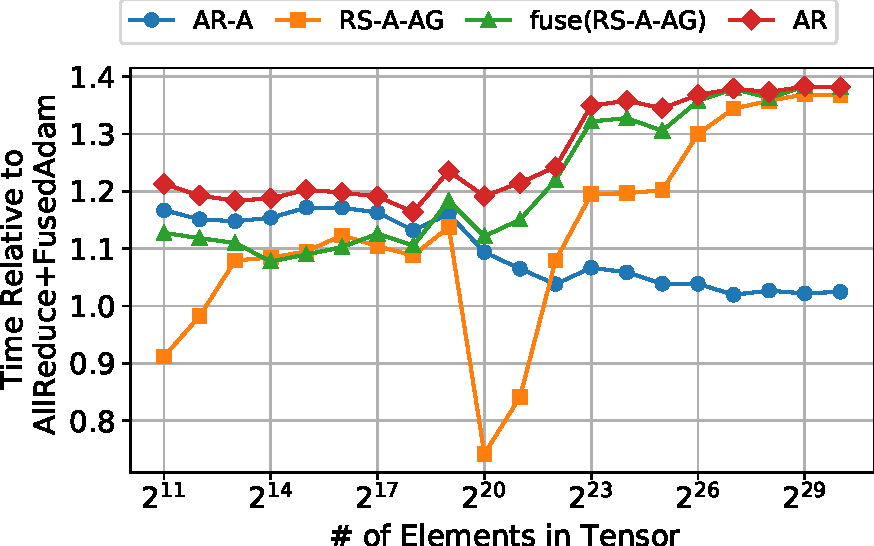
\includegraphics[width=\columnwidth]{figures/results-adam-64-gpus.pdf}  
    \caption{FP32 Adam on 64 GPUs}
  \end{subfigure}

  \begin{subfigure}{0.66\columnwidth}
    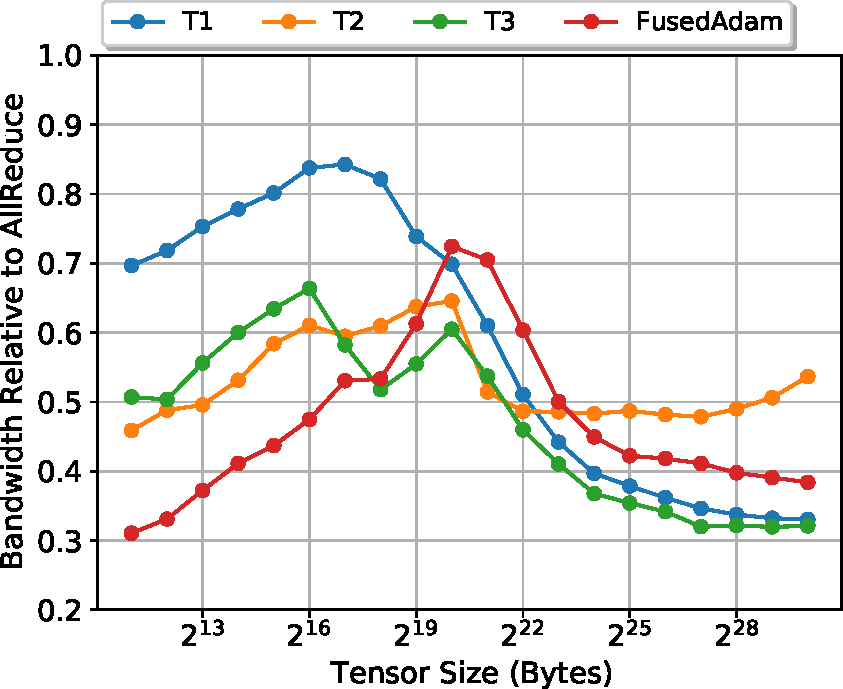
\includegraphics[width=\columnwidth]{figures/results-adamfp16-2-gpus.pdf} 
    \caption{MixedPrecision Adam on 2 GPUs} 
  \end{subfigure}
  \begin{subfigure}{0.66\columnwidth}
    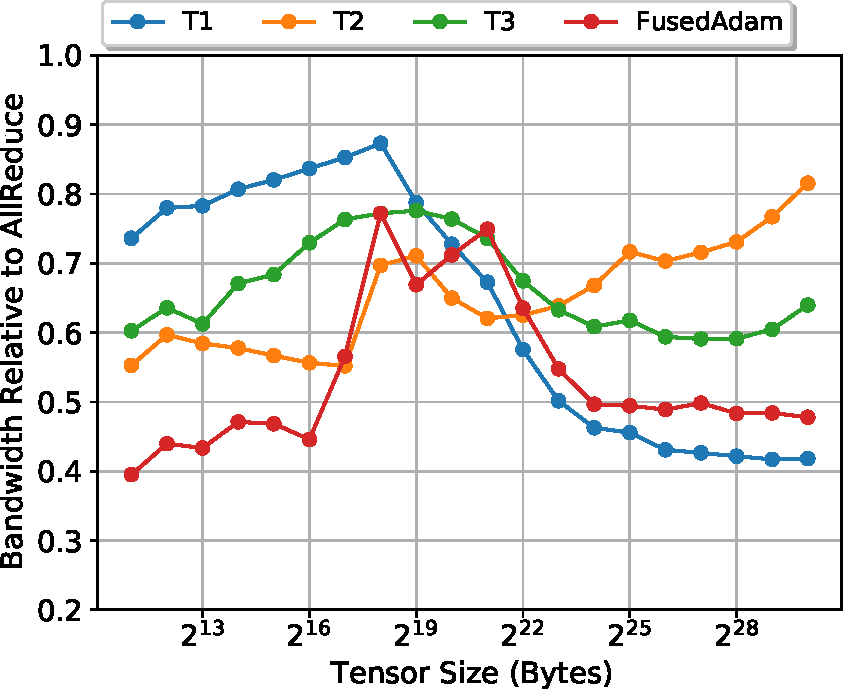
\includegraphics[width=\columnwidth]{figures/results-adamfp16-4-gpus.pdf}  
    \caption{MixedPrecision Adam on 4 GPUs} 
  \end{subfigure}
  \begin{subfigure}{0.66\columnwidth}
    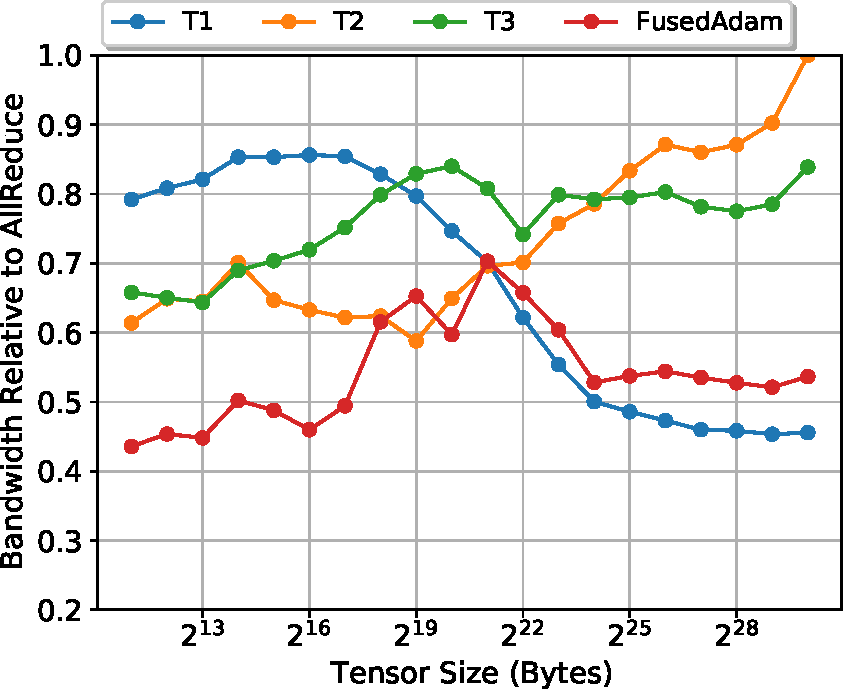
\includegraphics[width=\columnwidth]{figures/results-adamfp16-8-gpus.pdf} 
    \caption{MixedPrecision Adam on 8 GPUs} 
  \end{subfigure}

  \begin{subfigure}{0.66\columnwidth}
    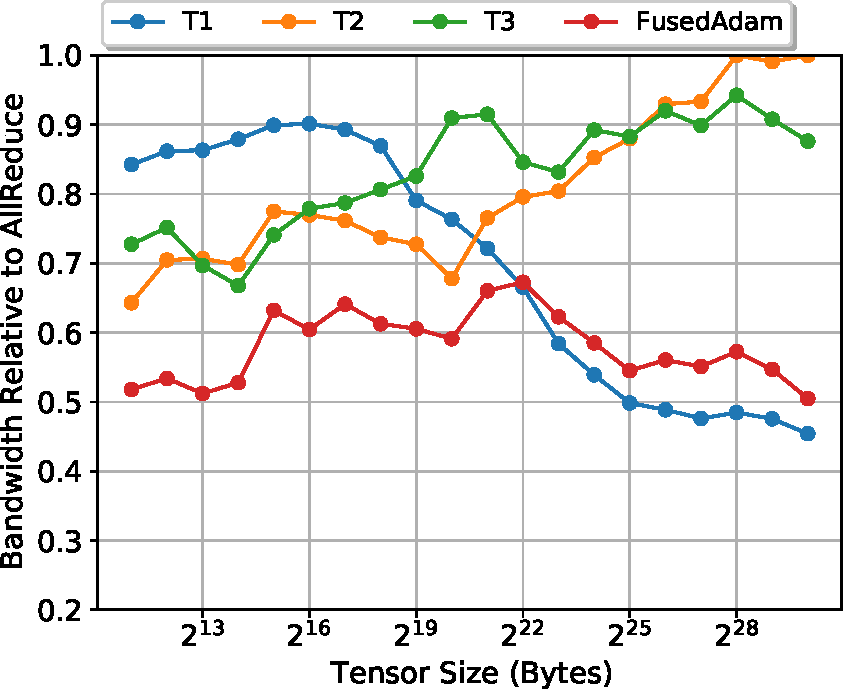
\includegraphics[width=\columnwidth]{figures/results-adamfp16-16-gpus.pdf} 
    \caption{MixedPrecision Adam on 16 GPUs} 
  \end{subfigure}
  \begin{subfigure}{0.66\columnwidth}
    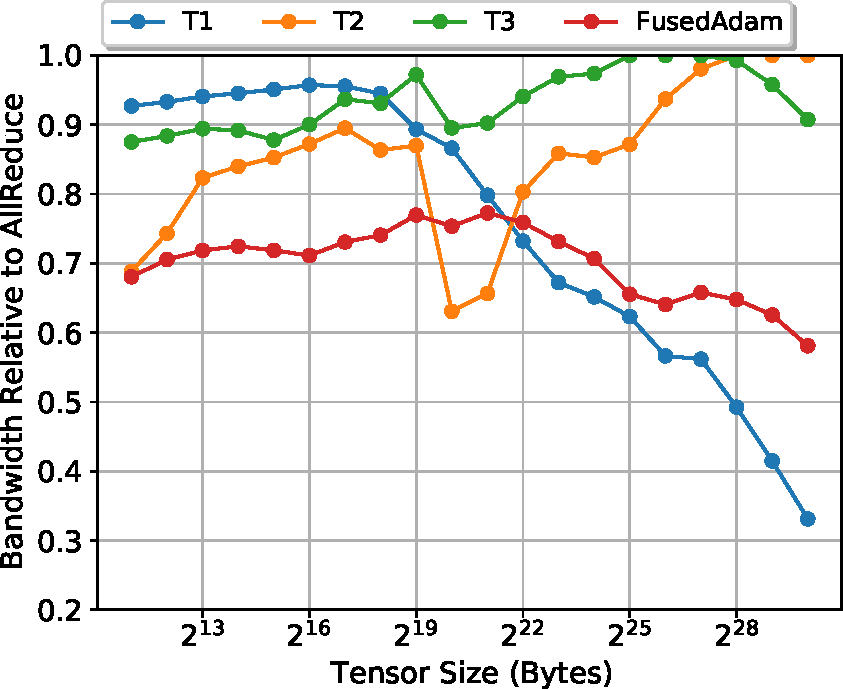
\includegraphics[width=\columnwidth]{figures/results-adamfp16-32-gpus.pdf}  
    \caption{MixedPrecision Adam on 32 GPUs} 
  \end{subfigure}
  \begin{subfigure}{0.66\columnwidth}
    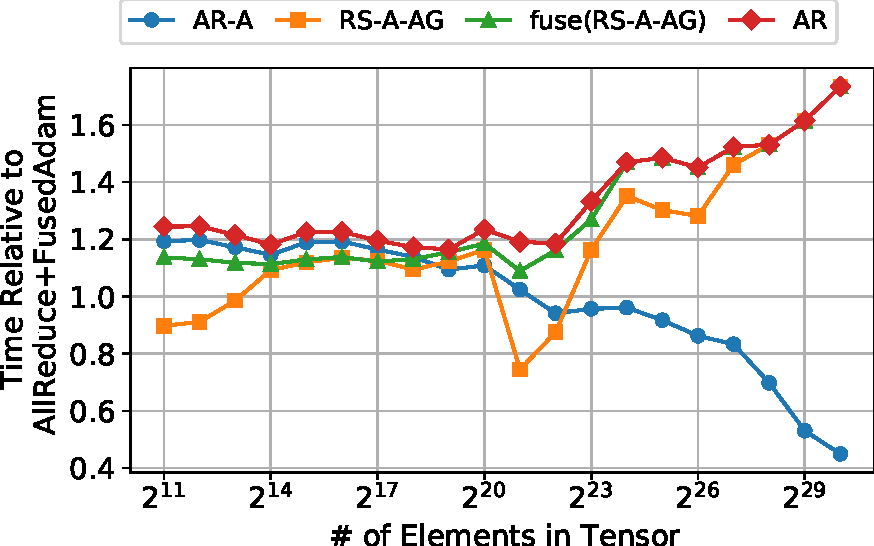
\includegraphics[width=\columnwidth]{figures/results-adamfp16-64-gpus.pdf} 
    \caption{MixedPrecision Adam on 64 GPUs} 
  \end{subfigure}
  \caption{Speedup of \tool s Adam vs FusedAdam (y-axis) against
    NVIDIA's handwritten apex library as a function of tensor size
    (x-axis). \aj{Instead of speedups show bandwidth obtained as compared to maximum bandwidth.} \label{fig:dslvsfusedadam}}
\end{figure*}

\begin{figure*}
  \small
  \begin{subfigure}{0.66\columnwidth}
    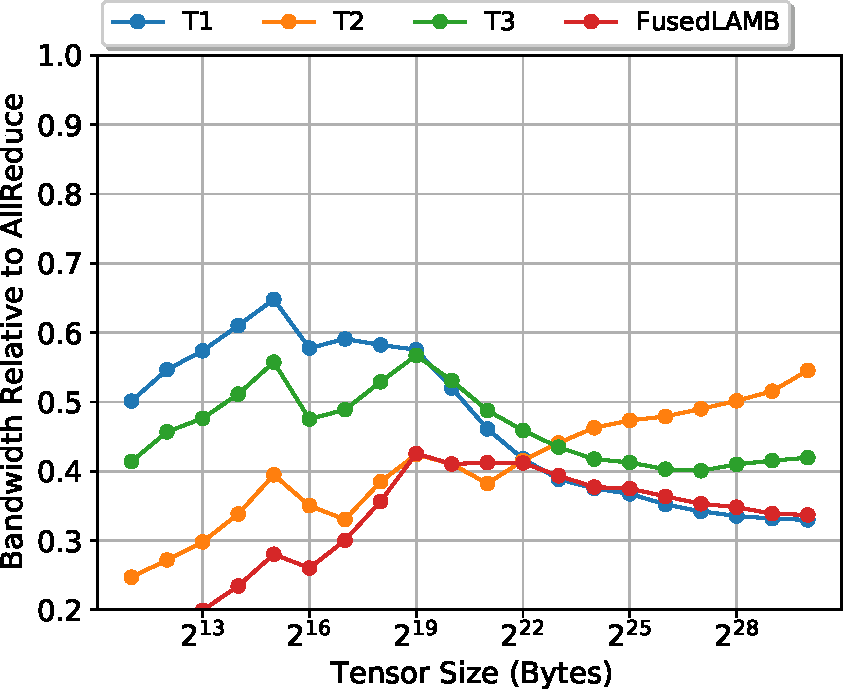
\includegraphics[width=\columnwidth]{figures/results-lamb-2-gpus.pdf}  
    \caption{FP32 LAMB on 2 GPUs}
  \end{subfigure}
  \begin{subfigure}{0.66\columnwidth}
    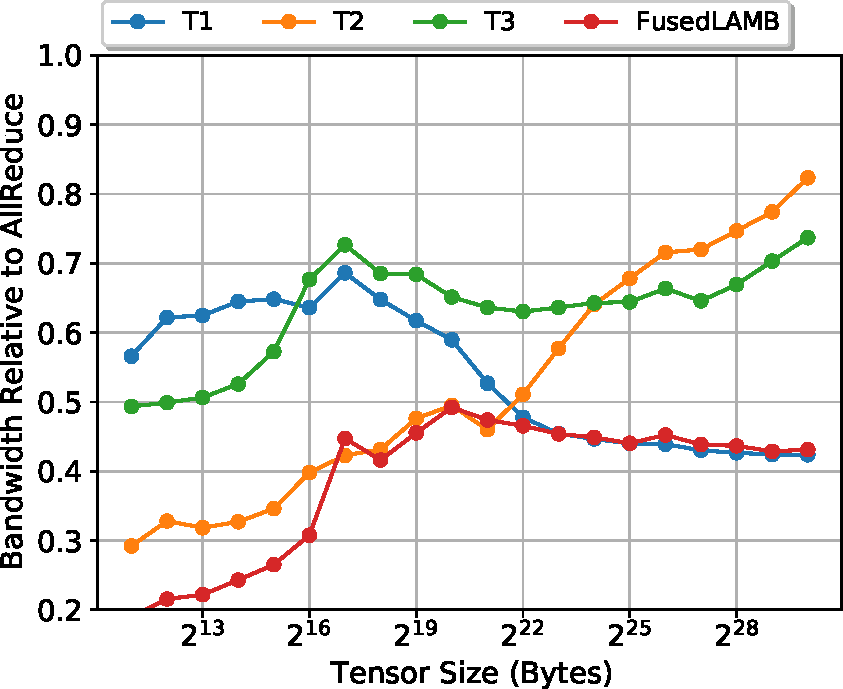
\includegraphics[width=\columnwidth]{figures/results-lamb-4-gpus.pdf}  
    \caption{FP32 LAMB on 4 GPUs}
  \end{subfigure}
  \begin{subfigure}{0.66\columnwidth}
    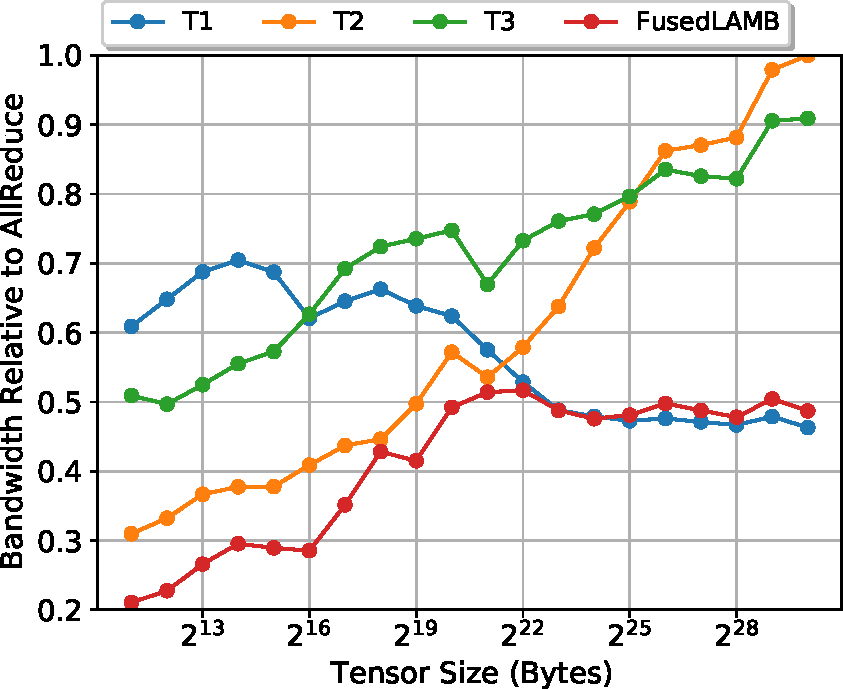
\includegraphics[width=\columnwidth]{figures/results-lamb-8-gpus.pdf}  
    \caption{FP32 LAMB on 8 GPUs}
  \end{subfigure}

  \begin{subfigure}{0.66\columnwidth}
    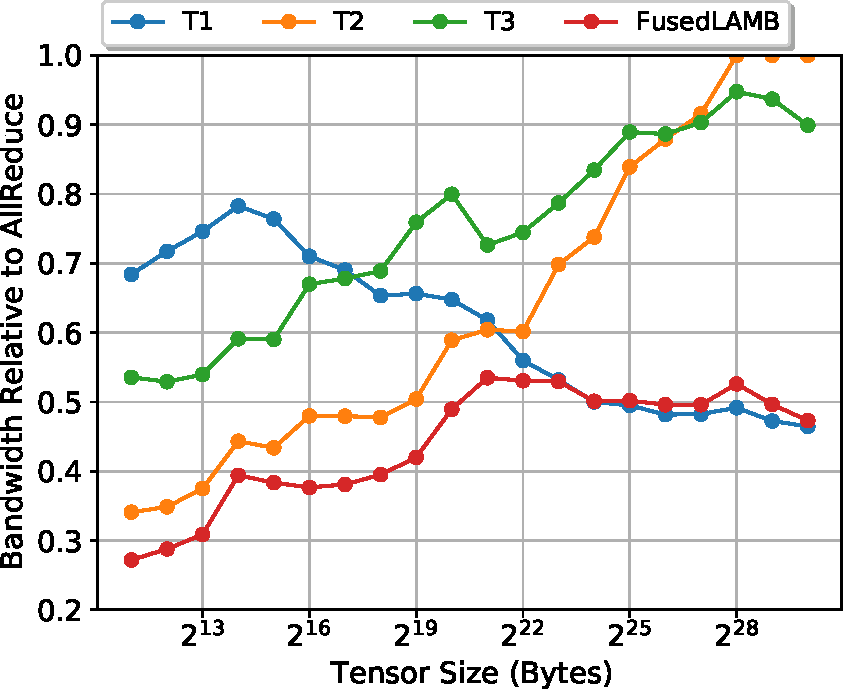
\includegraphics[width=\columnwidth]{figures/results-lamb-16-gpus.pdf}  
    \caption{FP32 LAMB on 16 GPUs}
  \end{subfigure}
  \begin{subfigure}{0.66\columnwidth}
    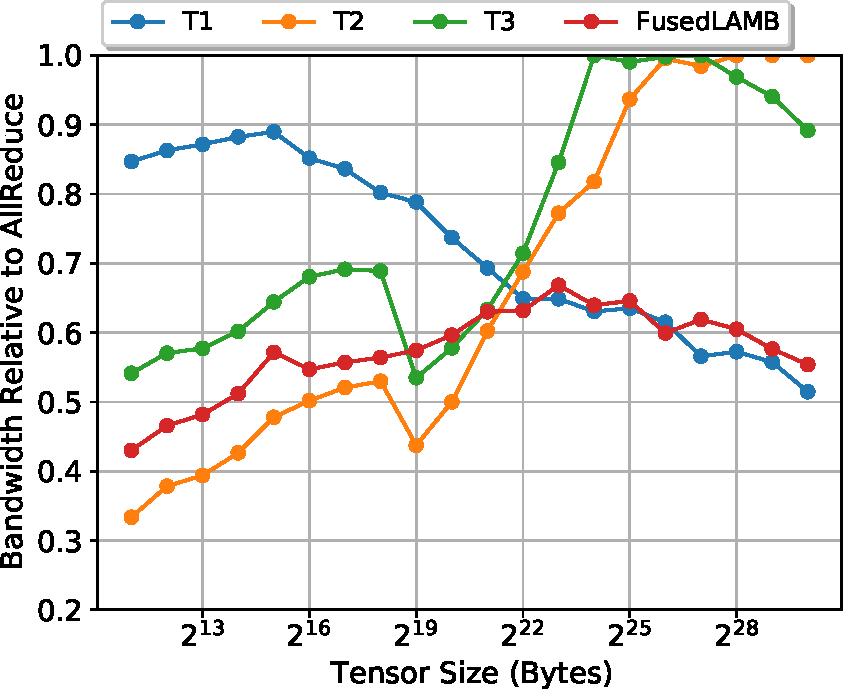
\includegraphics[width=\columnwidth]{figures/results-lamb-32-gpus.pdf}  
    \caption{FP32 LAMB on 32 GPUs}
  \end{subfigure}
  \begin{subfigure}{0.66\columnwidth}
    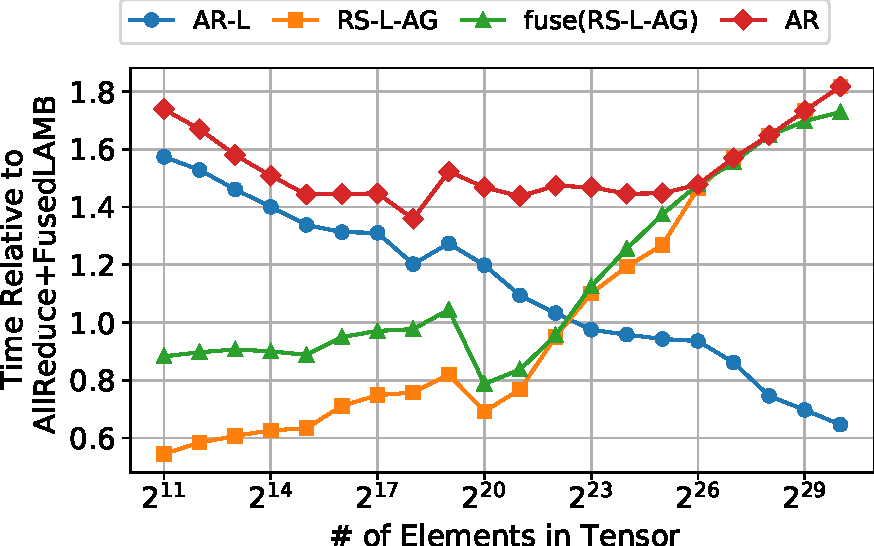
\includegraphics[width=\columnwidth]{figures/results-lamb-64-gpus.pdf}  
    \caption{FP32 LAMB on 64 GPUs}
  \end{subfigure}
  

  \begin{subfigure}{0.66\columnwidth}
    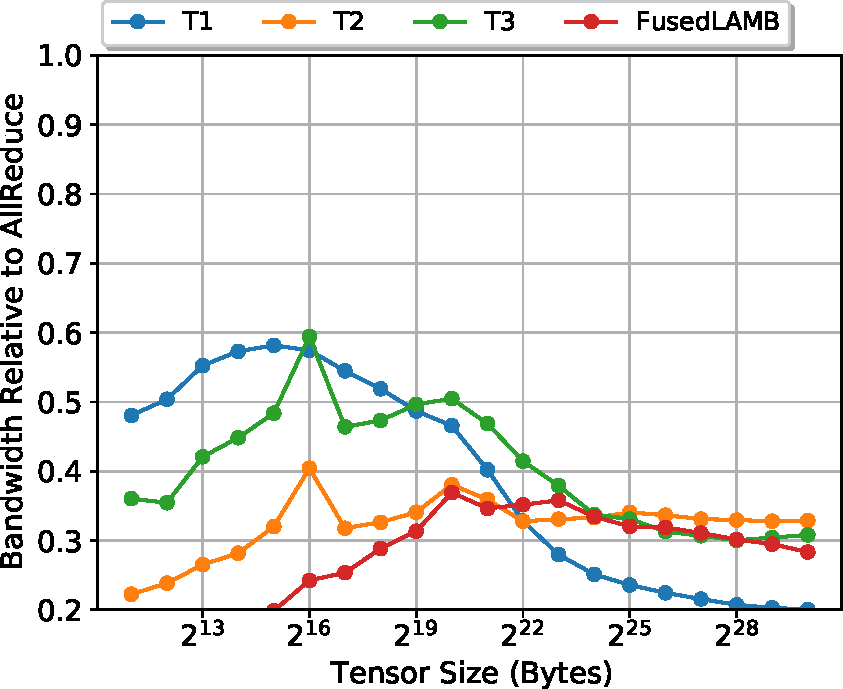
\includegraphics[width=\columnwidth]{figures/results-lambfp16-2-gpus.pdf} 
    \caption{MixedPrecision LAMB on 2 GPUs} 
  \end{subfigure}
  \begin{subfigure}{0.66\columnwidth}
    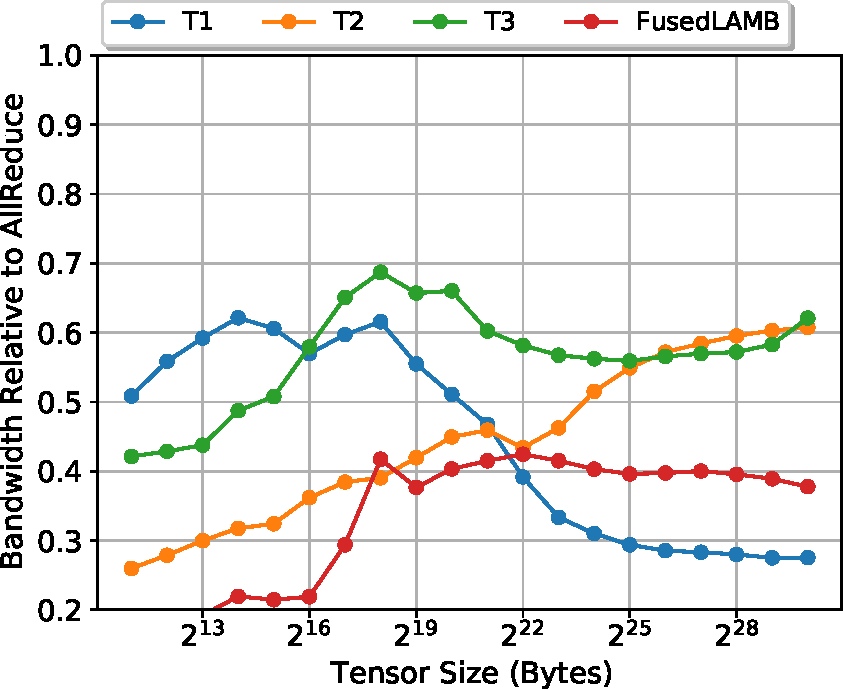
\includegraphics[width=\columnwidth]{figures/results-lambfp16-4-gpus.pdf}  
    \caption{MixedPrecision LAMB on 4 GPUs} 
  \end{subfigure}
  \begin{subfigure}{0.66\columnwidth}
    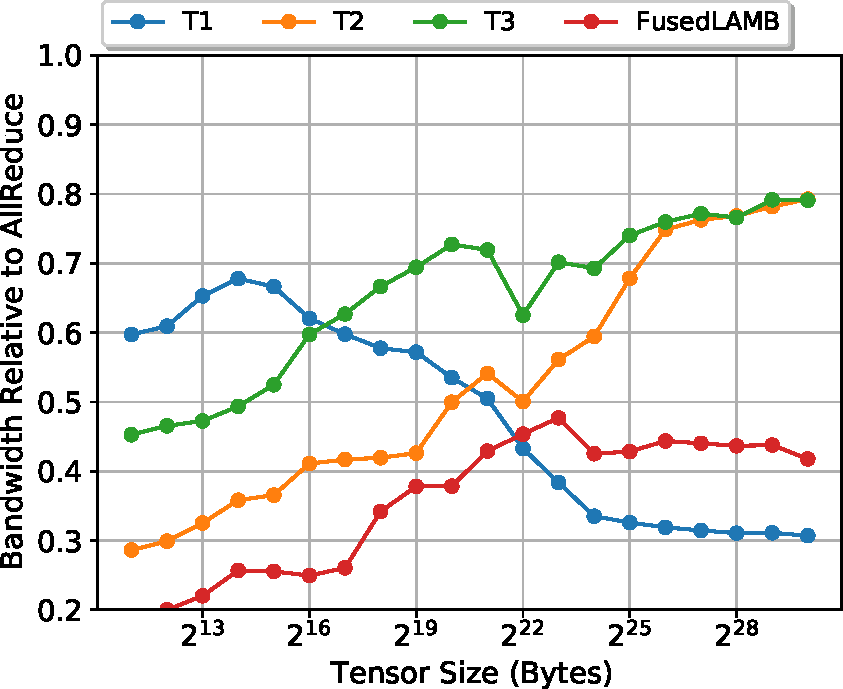
\includegraphics[width=\columnwidth]{figures/results-lambfp16-8-gpus.pdf}  
    \caption{MixedPrecision LAMB on 8 GPUs}
  \end{subfigure}

  \begin{subfigure}{0.66\columnwidth}
    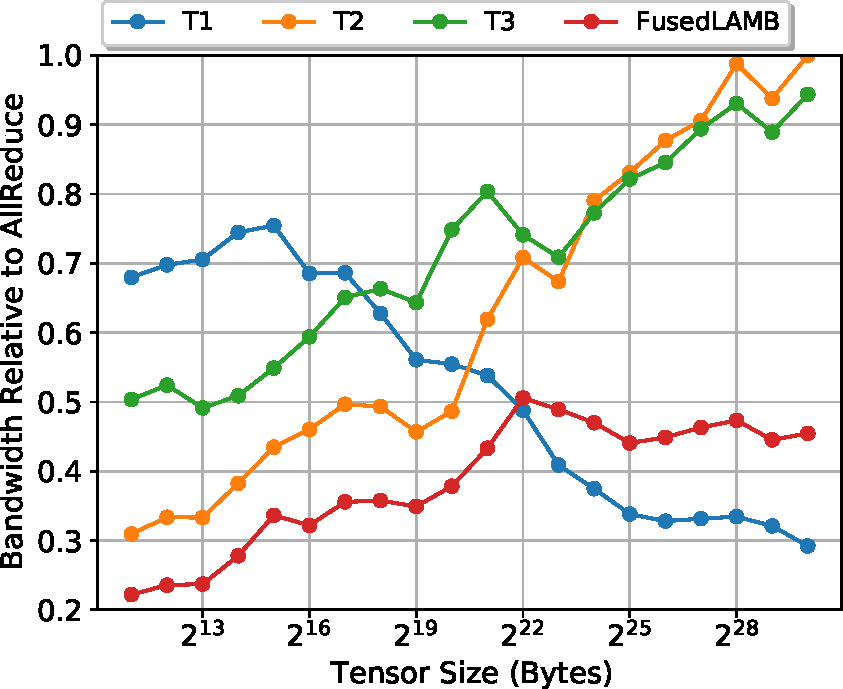
\includegraphics[width=\columnwidth]{figures/results-lambfp16-16-gpus.pdf} 
    \caption{MixedPrecision LAMB on 16 GPUs} 
  \end{subfigure}
  \begin{subfigure}{0.66\columnwidth}
    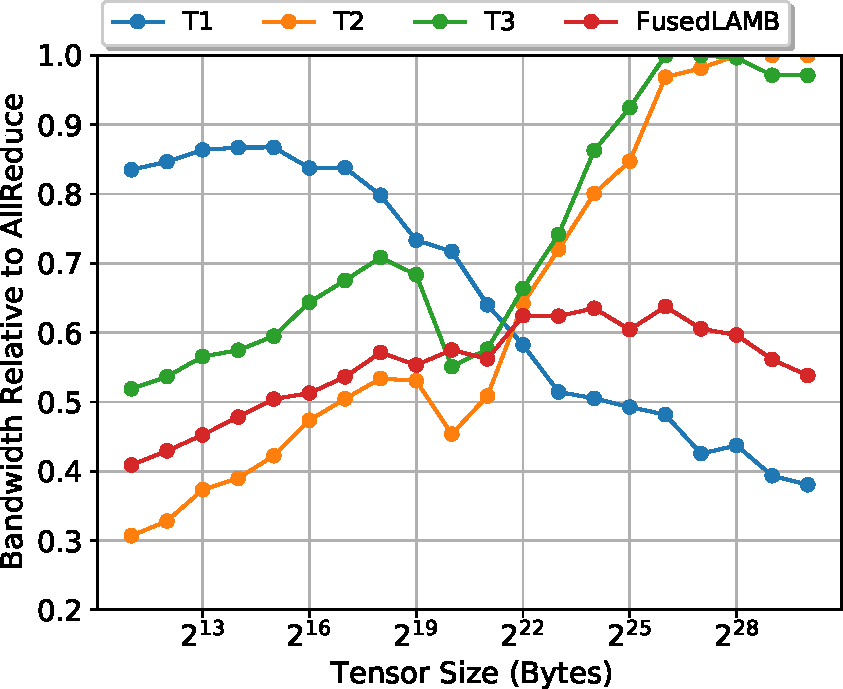
\includegraphics[width=\columnwidth]{figures/results-lambfp16-32-gpus.pdf}  
    \caption{MixedPrecision LAMB on 32 GPUs} 
  \end{subfigure}
  \begin{subfigure}{0.66\columnwidth}
    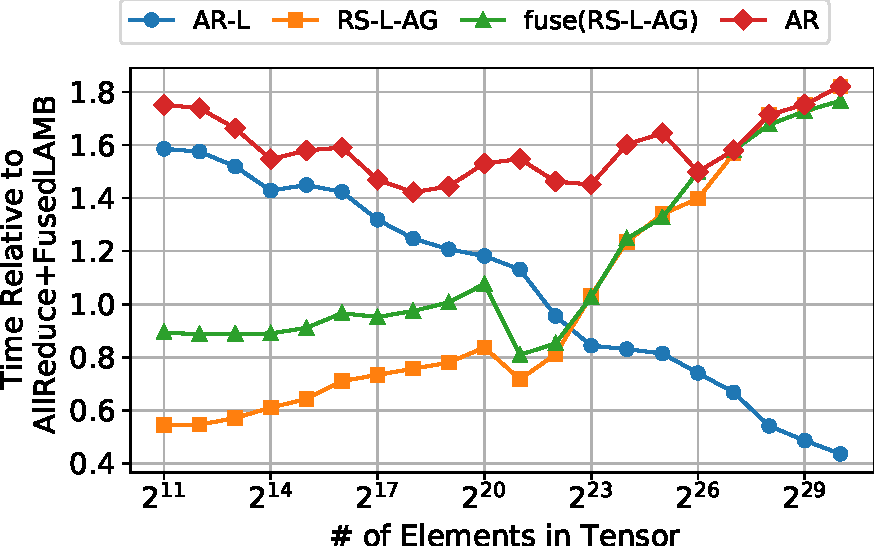
\includegraphics[width=\columnwidth]{figures/results-lambfp16-64-gpus.pdf}  
    \caption{MixedPrecision LAMB on 64 GPUs} 
  \end{subfigure}
  \caption{Speedup of \tool s LAMB vs FusedLAMB (y-axis) against
    NVIDIA's handwritten apex library as a function of tensor size
    (x-axis). \label{fig:speedupsVSapex}}
\end{figure*}
\fi
 
\begin{table}
  \centering
	\small
  \caption{Lines of code of implementation of distributed machine learning workloads in CUDA and \tool{}, and time taken by the autotuner to find the best schedule.}
  \label{tab:loc-autotuner-time}

  \begin{subtable}{\linewidth}
    \centering
    \caption{Data Parallel optimizer update using Adam and LAMB\label{tab:loc:data-parallel}}
  \begin{tabular}{lrrr}
    \textbf{Schedule}        & \textbf{\thead{Generated\\CUDA}} & \textbf{\thead{Program in\\\tool{}}} & \textbf{\thead{Autotuner\\Time}}\\ \hline
    \textit{AR-Adam}           & 16   &  12  & \multirow{3}{*}{9 secs}    \\
    \textit{RS-Adam-AG}        & 24   &  16  &  \\
  \textit{fuse(RS-Adam-AG)}  & 150  &  17  & \\\hline
  \textit{AR-LAMB}           & 80   &  15  & \multirow{3}{*}{10 secs}   \\
  \textit{RS-LAMB-AG}        & 140  &  17  &   \\
  \textit{fuse(RS-LAMB-AG)}  & 220  &  18  & \\
  \hline
  \end{tabular}
  \par \bigskip% Do not remove this. Without this there is no space between caption and the table
  \end{subtable}

  \begin{subtable}{\linewidth}
    \centering
    \caption{Model Parallel Self Attention and Multi Layer Perceptron\label{tab:loc:model-parallel}}
  \begin{tabular}{lrrr}
    \textbf{Schedule}       & \textbf{\thead{Generated\\CUDA}} & \textbf{\thead{Program in\\\tool{}}} & \textbf{\thead{Autotuner\\Time}}\\ \hline
    \textit{MM-AR-C}               &  20  &  10   & \multirow{3}{*}{12 secs} \\
  \textit{MM-RS-C-AG}            &  140 &  13    & \\
  \textit{ol(MM,fuse(RS-C-AG))}  &$\approx$ 2k    &   14  &   \\\hline
  \end{tabular}
  \par \bigskip% Do not remove this. Without this there is no space between caption and the table
  \end{subtable}

  \begin{subtable}{\linewidth}
    \centering
    \caption{Pipeline Parallel Transformer Layer\label{tab:loc:pipeline-parallel}}
  \begin{tabular}{lrrr}
    \textbf{Schedule} & \textbf{\thead{Generated\\CUDA}} & \textbf{\thead{Program in\\\tool{}}} & \textbf{\thead{Autotuner\\Time}}\\ \hline
    \textit{AR-P2P-C-AG}               &  20  &  10  & \multirow{3}{*}{11 secs}  \\
    \textit{RS-P2P-C-AG}            &  140 &  13    & \\
    \textit{ol(RS,fuse(P2P-C),AG))}  &$\approx$ 2k    &   14  &   \\\hline
  \end{tabular}
  \par \bigskip% Do not remove this. Without this there is no space between caption and the table
  \end{subtable}
\end{table}

\subsubsection{Integeration with BERT}
\label{sec:experiments:bert}
We use \tool generated optimizers to train three large BERT models from NVIDIA~\cite{nvbert}.
We use mixed precision training with both Adam with 8192 global batch size and LAMB with 65536 global batch size.

\spara{Baselines} We consider three baselines for this experiment:
\begin{itemize}
  \item \textbf{NV BERT}~\cite{nvbert} is the NVIDIA BERT Script. 
  It copies gradients of each layer into a single buffer, calls \allreduce on the buffer, and
  copy back the results into original gradients. Finally, it calls either FusedAdam or FusedLAMB.
  \item \textbf{PyTorch DDP}~\cite{pytorch-ddp} stores all gradients in buckets of 25MB and overlaps the \allreduce on each gradient bucket with computations during training. After reducing all gradients it calls FusedAdam or FusedLAMB.
  \item \textbf{ZeRO}~\cite{zero}
  copies gradients into a contiguous buffer and then distributes Adam's computation similar to \textit{RS-Opt-AG} schedules above.
  The ZeRO implementation of LAMB does not support distributing optimizer state among GPUs because significant engineering efforts are required to implement reduction over distributed gradients and weights in a distributed LAMB implementation~\cite{deepspeed490}.
%  \footnote{https://github.com/microsoft/DeepSpeed/issues/490}
  % \tool generates scattered tensors implementation for both Adam and LAMB.
\end{itemize}

\spara{\tool Integeration} We integrated the scattered tensors implementation of \textit{fuse(RS-Opt-AG)} schedule for both Adam and LAMB in PyTorch. 
These implementations provide three benefits over the baselines: (i) the scattered tensor implementation avoids copying all gradients to a single buffer and allocating this buffer, (ii) the fused schedule performs best for the tensor sizes used in BERT, and (iii) the fused schedule distributes memory of optimizer state among all GPUs.

\begin{table*}
	\small
  \centering
  \caption{Maximum Micro Batch Size supported by all implementations and speedup of \tool over the baselines when training BERT with three parameter configurations using Adam and LAMB optimizer. OOM represents Out of Memory.\label{tab:bert-results}}
  \begin{tabular}{cccccccccccc}
  \textbf{Optimizer} & \textbf{\# of Parameters} & \multicolumn{4}{c}{\textbf{Maximum Micro Batch Size}} & \multicolumn{3}{c}{\textbf{Speedup of \tool over}}\\
  \cmidrule(lr){3-6} \cmidrule(lr){7-9}
                          & & NV BERT & PyTorch DDP & ZeRO & \tool & NV BERT & PyTorch DDP & ZeRO  \\
  \hline
  \multirow{3}{*}{Adam} & 336 M & 32  &  32  & 32 & 32 & 1.18$\times$ & 1.22$\times$ & 1.10$\times$\\ 
  &1.2 B & 8   &  8   & 32 & 32 & 1.53$\times$ & 1.52$\times$ & 1.10$\times$\\ 
  &3.9 B & OOM & OOM & 8  & 8 & -- & -- & 1.22$\times$\\
  \hline
  \multirow{3}{*}{LAMB} & 336M & 64 & 64 & 64 &128 & 1.20$\times$ & 1.20$\times$ & 1.15$\times$\\
  & 1.2B & 8 & 8 & 8 & 64 &1.67$\times$ & 1.68$\times$ & 1.64$\times$\\ 
  & 3.9B & OOM & OOM & OOM & 8 & -- & -- & --\\ 
  \hline
  \end{tabular}
  \par \bigskip% Do not remove this. Without this there is no space between caption and the table
\end{table*}

% \begin{table*}
% 	\small
%   \begin{subtable}{0.463\linewidth}  
%   \begin{tabularx}{\textwidth}{|l|r|r|r|}
%     \hline
%     \textbf{Schedule}        & \textbf{CUDA} & \textbf{\tool{}} & \textbf{\thead{Autotuning\\Time(secs)}}\\ \hline
%   AR-Adam           & 16   &  12  & \multirow{3}{*}{10}    \\
%   RS-Adam-AG        & 24   &  16  &  \\
%   fuse(RS-Adam-AG)  & 150  &  17  & \\\hline
%   AR-LAMB           & 80   &  15  & \multirow{3}{*}{10}   \\
%   RS-LAMB-AG        & 140  &  17  &   \\
%   fuse(RS-LAMB-AG)  & 220  &  18  & \\
%   \hline
%   \end{tabularx}
%   \caption{Data Parallel optimizer update using Adam and LAMB\label{tab:loc:data-parallel}}
%   \end{subtable}
%   \hfill
%   \begin{subtable}{0.504\linewidth}
%   \begin{tabularx}{\textwidth}{|l|r|r|r|}
%     \hline
%     \textbf{Schedule}       & \textbf{CUDA} & \textbf{\tool{}} & \textbf{\thead{Autotuning\\Time(secs)}}\\ \hline
%   MM+AR+C               &  20  &  10   & \multirow{3}{*}{10} \\
%   MM+RS+C+AG            &  140 &  13    & \\
%   OL(MM,fuse(RS+C+AG))  &$\approx$ 2k    &   14  &   \\\hline
%   \end{tabularx}
%   \caption{Model Parallel Self Attention and Multi Layer Perceptron\label{tab:loc:model-parallel}}

%   \begin{tabularx}{0.904\textwidth}{|l|r|r|r|}
%     \hline
%     \textbf{Schedule} & \textbf{CUDA} & \textbf{\tool{}} & \textbf{\thead{Autotuning\\Time(secs)}}\\ \hline
%   AR+P2P+C+AG               &  20  &  10  & \multirow{3}{*}{10}  \\
%   RS+P2P+C+AG            &  140 &  13    & \\
%   OL(RS,P2P+C,AG))  &$\approx$ 2k    &   14  &   \\\hline
%   \end{tabularx}
%   \caption{Pipeline Parallel Transformer Layer\label{tab:loc:pipeline-parallel}}
%   \end{subtable}
%   \caption{Lines of code of implementation of distributed machine learning workloads in CUDA and \tool{}, and time taken by the autotuner to find best schedule for each workload.}
% \end{table*}

\spara{Results} Table~\ref{tab:bert-results} shows the speedup provided by \tool in training three BERT models over baselines.
For Adam optimizer, \tool provides speedup over all baselines in training BERT 336M because \tool's fused schedules perform better than other implementations.
\tool provides even higher speedup on larger BERT models because the fused schedules decrease memory usage by distributing Adam's state over all GPUs, which improves the efficiency of matrix multiplication GPU kernels by enabling higher batch size per iteration.
For example, for BERT 1.2B \tool provides 1.53$\times$ speedup over NV BERT and PyTorchDDP because of the optimized fused schedule and higher batch size enabled by \tool.
On 3.9B parameter model, NV BERT and PyTorch go Out of Memory.
ZeRO also supports higher batch size for BERT 1.2B and 3.9B but \tool still gives speedup because of the advantages of scattered tensor implementation of fused schedules.

Results for LAMB are similar. 
\tool provides up to 1.64$\times$ speedup over all baselines. 
For LAMB, the speedup over ZeRO is higher than Adam because ZeRO does not support distributing LAMB optimizer state, and hence, supports smaller batch sizes as compared to \tool.
% For example, \tool provides upto 1.68$\times$ speedup over all baselines because it supports batch size of 64 while baselines have a maximum batch size of 8. 

In summary, \tool significantly improves data-parallel training time of BERT models. 
\tool's schedules can be automatically generated and \tool's scattered tensors implementation can support a  wide range of optimizers.
Not only does the fusion of computation and communication lead to performance improvement over the baselines of PyTorch DDP and ZeRO, it also decreases the memory usage, which helps in increasing the batch size to train models faster.
% \spara{BERT baseline} To avoid invoking \allreduce for each layer separately, the original model script allocates a single buffer that can hold gradients for all model parameters.
% After each backward pass, it uses Apex~\cite{apex} to copy all gradients into the buffer and then calls \allreduce on the buffer. 
% After \allreduce the model script again uses Apex to copy the gradients back to their original tensors and calls Apex's FusedAdam.

%Micro Batch Size = (Total Batch Size)/((Number of GPUs) * (Gradient Accumulation Steps))

%Micro Batch Size and times for Adam
% \begin{table*}
% 	\small
%   \begin{tabular}{@{}c|c|c|c|c@{}|c|c|c|c|c|c|c}
%   \textbf{BERT Parameters} & \multicolumn{2}{c|}{\textbf{Baseline}} & \multicolumn{2}{c|}{\textbf{PyTorch DDP}} & \multicolumn{2}{c|}{\textbf{ZeRO}} & \multicolumn{2}{c|}{\textbf{\tool}}\\
%                            & Micro Batch Size & Time & Micro Batch Size & Time & Micro Batch Size & Time & Micro Batch Size & Time \\
%   \hline
%   336 M & 32  & 0.245  & 32  & 0.257 & 32 & 0.233& 32 & 0.211\\ 
%   1.2 B & 8   & 0.89 & 8   &0.88 & 64 & 0.70& 64 & 0.58 \\ 
%   3.9 B & OOM & -- & OOM & -- & 8  & 1.68 & 8  & 1.37 \\
%   \end{tabular}
%   \caption{Adam with Global Batch Size 8192.}
% \end{table*}

% %Micro Batch Size and times for LAMB
% \begin{table*}
% 	\small
%   \begin{tabular}{@{}c|c|c|c|c@{}|c|c|c|c|c|c}
%     \textbf{BERT Parameters} & \multicolumn{2}{c}{\textbf{Baseline}} & \multicolumn{2}{c}{\textbf{PyTorch DDP}} & \multicolumn{2}{c}{\textbf{ZeRO}} & \multicolumn{2}{c}{\textbf{\tool}}\\
%     & Micro Batch Size & Time & Micro Batch Size & Time & Micro Batch Size & Time & Micro Batch Size & Time \\
%   \hline
%   336 M & 64  & 1.62 & 64  & 1.61 & 64  & 1.49 & 128 & 1.35\\ 
%   1.2 B & 8   & 5.8 & 8   & 5.9 & 8   & 5.6 & 64  & 3.5\\ 
%   3.9 B & OOM & -- & OOM & -- & OOM & -- & 8   & 8.41\\
%   \end{tabular}
%   \caption{LAMB with Global Batch Size 65536}
% \end{table*}


% \begin{table*}
% 	\footnotesize
%   \begin{tabularx}{0.6\textwidth}{c@{}c@{}c@{}c@{}c@{}c@{}c@{}c@{}c@{}c@{}c@{}c@{}c@{}c@{}c@{}c@{}}
%   \textbf{\# of Params} & \multicolumn{7}{c}{Adam} & \multicolumn{7}{c}{LAMB}\\
%   & \multicolumn{4}{c}{\textbf{Micro Batch Size}} & \multicolumn{3}{c}{\textbf{Speedup of \tool over}} & \multicolumn{4}{c}{\textbf{Micro Batch Size}} & \multicolumn{3}{c}{\textbf{Speedup of \tool over}}\\
%   \cmidrule(lr){2-5} \cmidrule(lr){6-8}
%                            & Baseline & PyTorch & ZeRO & \tool & Baseline & PyTorch & ZeRO  & Baseline & PyTorch & ZeRO & \tool & Baseline & PyTorch & ZeRO  \\
%   \hline
%   336 M & 32  &  32  & 32 & 32 & 1.16$\times$ & 1.22$\times$ & 1.10$\times$\\ 
%   1.2 B & 8   &  8   & 32 & 32 & 1.53$\times$ & 1.52$\times$ & 1.10$\times$\\ 
%   3.9 B & OOM & OOM & 8  & 8 & -- & -- & 1.22$\times$\\
%   \hline
%   336M & 64 & 64 & 64 &128 & 1.20$\times$ & 1.20$\times$ & 1.10$\times$\\
%   1.2B & 8 & 8 & 8 & 64 &1.67$\times$ & 1.68$\times$ & 1.59$\times$\\ 
%   3.9B & OOM & OOM & OOM & 8 & -- & -- & --\\ 
%   \hline
%   \end{tabularx}
%   \caption{}
% \end{table*}

%Micro Batch Size and times for LAMB
% \begin{table*}
% 	\small
%   \begin{tabularx}{\textwidth}{@{}c|c|c|c|c@{}|c|c|c|c|c|c}
%     \textbf{BERT Parameters} & \multicolumn{2}{c}{\textbf{Baseline}} & \multicolumn{2}{c}{\textbf{PyTorch DDP}} & \multicolumn{2}{c}{\textbf{ZeRO}} & \multicolumn{2}{c}{\textbf{\tool}}\\
%     & Micro Batch Size & Time & Micro Batch Size & Time & Micro Batch Size & Time & Micro Batch Size & Time \\
%   \hline
%   336 M & 64  & 1.62 & 64  & 1.61 & 64  & 1.49 & 128 & 1.35\\ 
%   1.2 B & 8   & 5.8 & 8   & 5.9 & 8   & 5.6 & 64  & 3.5\\ 
%   3.9 B & OOM & -- & OOM & -- & OOM & -- & 8   & 8.41\\
%   \end{tabularx}
%   \caption{LAMB with Global Batch Size 65536}
% \end{table*}

\subsection{Model Parallelism}
Megatron-LM~\cite{megatronlm} uses a model parallel approach for inference and training of transformer models, such as BERT~\cite{bert} and GPT-2~\cite{gpt-2}. 
A transformer layer contains a self-attention block and a 
multi-layer perceptron (MLP) block. Last few operations of a self-attention block are the same 
computations as shown in Figure~\ref{fig:traditional-mp}. An MLP block's last operations are similar to 
Figure~\ref{fig:traditional-mp} with the input tensor and weight sizes as $[B, S, 4 \times H]$ and $[4 \times H, H]$ ($B$, $S$, and $H$ are batch size, sequence length, and hidden size, respectively).
Since model parallelism is applied within one node, all experiments in this section are performed on a single NVIDIA DGX-2 node.

\subsubsection{Standalone Experiments}
We first perform standalone experiments to evaluate different schedules generated by the autotuner.
We compare following schedules for model parallel self-attention code of Figure~\ref{fig:traditional-mp} and similar operations of multi-layer perceptron:
\begin{enumerate}[leftmargin=*,topsep=2pt]
  \item \textbf{Megatron-LM} is the baseline implementation of Figure~\ref{fig:traditional-mp} in Megatron-LM.
  \item \textbf{MM-AR-C} improves the Megatron-LM implementation by fusing all pointwise computations into one kernel.
  \item \textbf{GShard-Eq} or \textbf{MM-RS-C-AG} uses the same techniques as GShard. It is generated from \textit{MM-AR-C} by splitting the \allreduce into a \reducescatter and an \allgather, and reorders \allgather with computations. 
  This schedule represents GShard because GShard is not available for GPUs.
  %  is similar to the schedule that will be generated by GShard~\cite{gshard} after sharding the output of matrix multiplication across all ranks.
  \item \textbf{ol(MM,fuse(RS-C-AG)} is generated from the previous schedule by fusing the \reducescatter, computation, and \allgather into a FusedAllReduce and then overlapping it with the MatMul. 
  The autotuner returned this as the best schedule and hence represents \tool in our results.
\end{enumerate}
\begin{figure}[t]
	\centering
  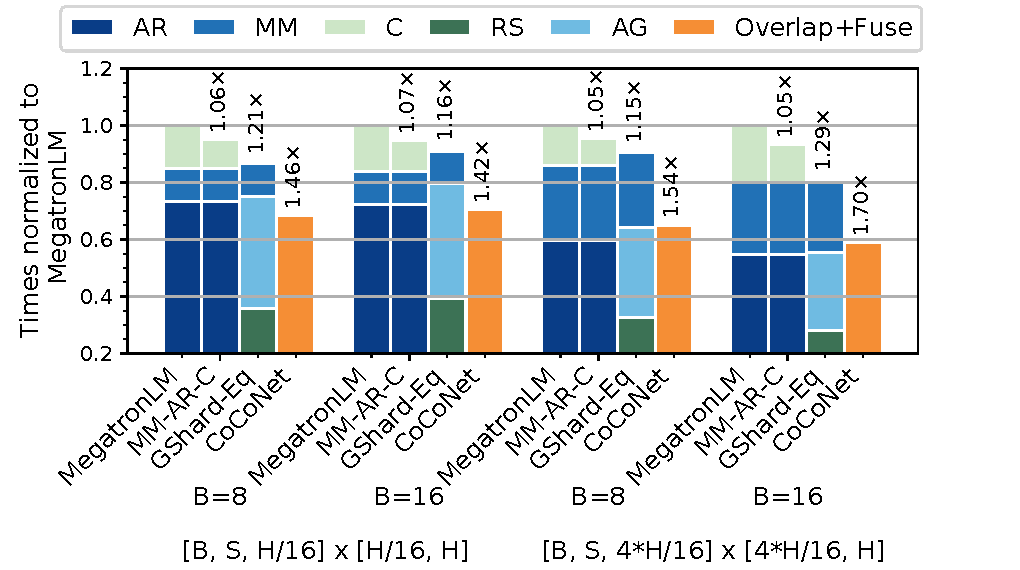
\includegraphics[width=\linewidth]{figures/matmul-overlap-16-gpus_combined.pdf}
  \caption{Times of \tool's schedules of model parallel self-attention and multi-layer perceptron of GPT-2 normalized to corresponding Megatron-LM's implementation.
  % Time spent in different kernels and speedup is shown for each schedule.
  \label{fig:matmul-overlap}}
\end{figure}

\spara{Results} We evaluate these schedules with sizes of GPT-2 8.3 Billion parameter model (i.e., $S=1024$, $H=3072$) for 8 and 16 batch sizes.
Figure~\ref{fig:matmul-overlap} shows the times of all schedules normalized to the time of implementation in Megatron-LM.
\textit{MM-AR-C} schedule provides speedup over Megatron-LM's implementation because this schedule fuses all pointwise computations in a single GPU kernel.
GShard-Eq (\textit{MM-RS-C-AG}) provides 1.15$\times$ to 1.29$\times$ speedup over Megatron-LM by distributing computations on all ranks.
\tool's best schedule (\textit{ol(MM,fuse(RS-C-AG))}) provides 1.42$\times$ to 1.70$\times$ speedup over Megatron-LM and 1.21$\times$ to 1.34$\times$ over GShard-Eq because it overlaps Fused\allreduce with the matrix multiplication.
Table~\ref{tab:loc:model-parallel} shows that the lines of generated CUDA code for each schedule are significantly more than the implementation in \tool and the autotuner explored all schedules in 12 seconds.

\subsubsection{Integration with Megatron-LM}
\label{sec:experiments:model-parallel:integeration}
After integrating \tool's overlap schedule in Megatron-LM,
we found that \tool improved inference times of BERT 3.9B parameter model by 1.51$\times$ and GPT-2 8.3B parameter model by 1.48$\times$.
Hence, overlapping matrix multiplication with fused collective communication significantly improves inference times.


\subsection{Pipeline Parallelism}
\tool can decrease inference times in pipeline parallelism by fusing computation and communication and overlapping multiple communication operations.
We evaluate \tool on computations of model and pipeline parallelism in Megatron-LM for GPT-2 8.3B and GPT-3 175B parameter models.
A transformer layer contains several operations but the operations of interest for this experiment are presented in Figure~\ref{fig:traditional-p2p}.
All experiments in this section are performed on all 16 NVIDIA DGX-2 nodes.

\subsubsection{Standalone Experiments}
We first perform standalone experiments to evaluate different schedules generated by the autotuner.
We compare the following schedules for pipeline parallelism code of Figure~\ref{fig:traditional-p2p}:
\begin{enumerate}[leftmargin=*,topsep=2pt]
 \item \textbf{Megatron-LM} is the implementation of Figure~\ref{fig:traditional-p2p} in Megatron-LM and serves as a baseline for this experiment.
 \item \textbf{AR-C-P2P-AG} is generated by slicing the output of \allreduce to perform sliced P2P sends and computations, and finally an \allgather to collect the output of computations.
 This schedule improves over Megatron-LM by slicing the P2P sends and fusing all the computations.
 \item \textbf{GShard-Eq} or \textbf{RS-C-P2P-AG} is generated from the previous schedule by splitting the \allreduce into a \reducescatter and an \allgather, then reordering the \allgather with P2P send and computations.
 Since this schedule is similar to GShard, it represents GShard-Eq in our results.
  \item \textbf{ol(RS,fuse(C-P2P),AG)} is generated from previous schedule by fusing computations with P2P sends, and overlapping all three communication operations (Figure~\ref{fig:p2p-fusion-3}). This schedule is returned by the autotuner as the best schedule and hence, represents \tool in our results.
\end{enumerate}

\spara{Results} 
Figure~\ref{fig:pipeline-overlap} shows the breakdown of each operation
with one transformer layer assigned to each node. The sequence length ($S=2048$) and the hidden
size ($H=12288$) are of GPT-3 175B model.
\tool's best schedule \textit{ol(RS,fuse(C-P2P),AG)} is 11.75$\times$--12.21$\times$ faster than Megatron-LM's implementation, 2.84$\times$ faster than \textit{AR-C-P2P-AG}, and 1.66$\times$--1.72$\times$ faster than GShard (\textit{RS-C-P2P-AG}). 
The speedups are because: 
(i) sliced P2P reduces cross node communication volume, 
(ii) fusing communication and computation operations improves memory bandwidth utilization, and
(iii) overlapping communication using different connections 
(NVLink within node and InfiniBand across nodes) improves network bandwidth utilization, while other schedules utilize only one stack at a time.
Table~\ref{tab:loc:pipeline-parallel} shows that the lines of generated CUDA code for each schedule are significantly more than the implementation in \tool and the autotuner explored all schedules in 11 seconds.

\subsubsection{Integration with Megatron-LM}
\label{sec:experiments:pipeline-parallel:integeration}
We evaluated the inference throughput of GPT-2 8.3B and GPT-3 175B parameter models by integrating \tool's \textit{ol(RS,fuse(C-P2P),AG)} schedule in Megatron-LM.
Table~\ref{tab:pipeline-results} shows the speedups achieved by \tool.
\begin{figure}[t]
	\centering
  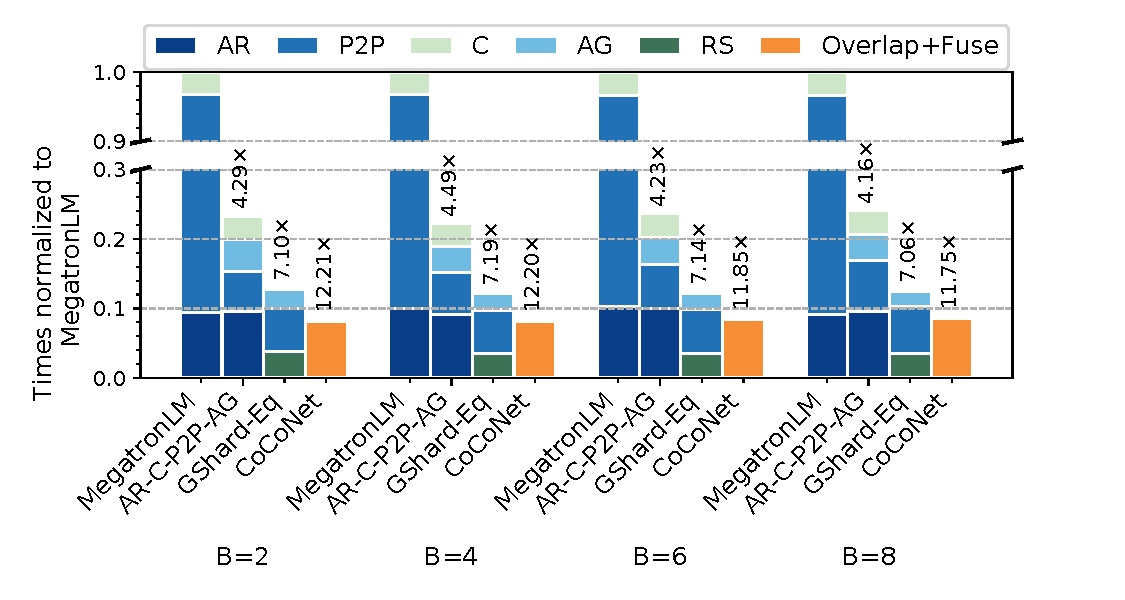
\includegraphics[width=1\linewidth]{figures/p2p-fusion-break-down-256-cluster_V100.pdf}
  \caption{Times of three schedules for GPT-3 175B in \tool for pipeline and model parallelism normalized to Megatron-LM's corresponding implementation. \label{fig:pipeline-overlap}}
\end{figure}

\tool significantly improves inference throughput of GPT-3 and GPT-2 due to its fusion and fine-grained overlapping of multiple communication operations.
% All these optimizations were possible only by breaking the computation and communication abstraction.
\begin{table}[t]
  \caption{Speedup in inference by \tool's implementation of pipeline parallelism for GPT-2 and GPT-3.
  Layers per node were obtained by equally distributing layers on all nodes.
  To evenly distribute layers of GPT-2, number of layers were increased to the nearest multiple of 16, i.e., 80.
  \label{tab:pipeline-results}}
  \begin{tabular}{lcccc}
    Model & \thead{Layers \\per node} & \thead{Maximum \\ Micro Batch Size} & Speedup \\
    \midrule
    GPT-2 8.3B & 5 & 16 & 1.77$\times$\\
    % GPT-3 175B & 1 & 8 & 2.45$\times$\\
    GPT-3 175B & 6 & 2 & 1.33$\times$\\
  \end{tabular} 
  \par \bigskip% Do not remove this. Without this there is no space between caption and the table
  \end{table}